% slides/problem_statement.tex

\begin{frame}
\frametitle{Arbitrary Image Style Transfer (AIST)}

\begin{itemize}
    \item \textbf{Definition:} Arbitrary Image Style Transfer (AIST) is the task of transferring the artistic style of one image (style image) onto another image (content image) while preserving the content of the original image.
    \item \textbf{Objective Function:}
    \[
    \mathcal{L} = \lambda_{\text{content}} \mathcal{L}_{\text{content}} + \lambda_{\text{style}} \mathcal{L}_{\text{style}}
    \]
    \begin{itemize}
        \item \(\mathcal{L}_{\text{content}}\): Content loss ensuring preservation of content features.
        \item \(\mathcal{L}_{\text{style}}\): Style loss ensuring accurate replication of style features.
        \item \(\lambda_{\text{content}}\) and \(\lambda_{\text{style}}\): Weighting factors balancing content and style contributions.
    \end{itemize}
    \item \textbf{Applications:}
    \begin{itemize}
        \item Creation of digital art and enhanced photography.
        \item Improving visual content for virtual and augmented reality environments.
        \item Automating design and image editing processes.
    \end{itemize}
\end{itemize}

\end{frame}

\begin{frame}
\frametitle{Challenges in Arbitrary Image Style Transfer}

\begin{itemize}
    \item \textbf{Content Preservation:} Ensuring that the essential structures and objects in the content image remain intact after style transfer.
    \item \textbf{Style Accuracy:} Precisely replicating the artistic style, including colors, textures, and brushstrokes, from the style image.
    \item \textbf{Scalability:} Enabling the model to handle an unlimited variety of styles without the need for separate models for each style.
    \item \textbf{Real-Time Performance:} Achieving fast processing speeds suitable for applications requiring instant style transfer, such as mobile apps and interactive systems.
    \item \textbf{Artifact Minimization:} Reducing visual artifacts and inconsistencies that may arise during the style transfer process.
\end{itemize}

\end{frame}

\begin{frame}
\frametitle{RAST Architecture Overview}

\begin{figure}[H]
    \centering
    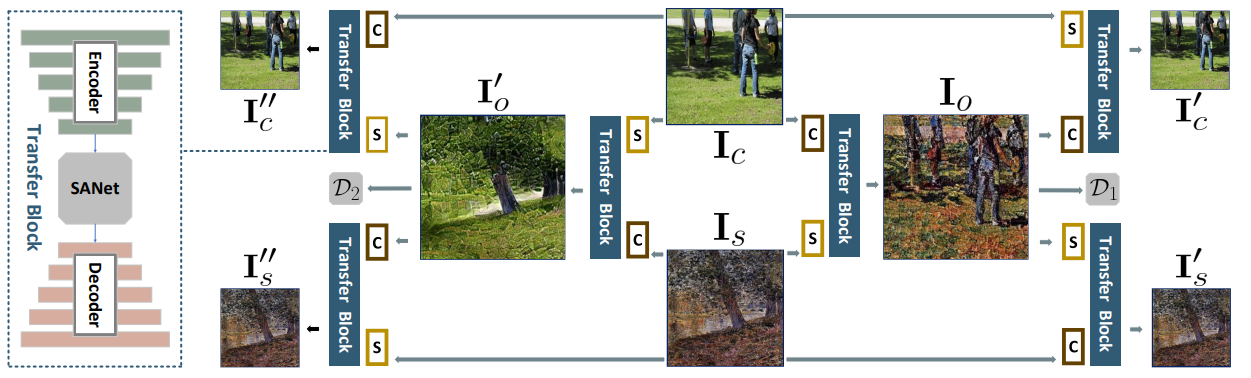
\includegraphics[width=0.8\textwidth]{figures/rast_architecture_overview.png} % Ensure this image exists in your 'figures' folder
    \caption{Overview of the RAST Architecture}
    \label{fig:rast_architecture_overview}
\end{figure}

\end{frame}

\begin{frame}
\frametitle{RAST Objective Function}

\begin{itemize}
    \item \textbf{Overall Objective:}
    \[
        \mathcal{L} = \lambda_{contra} L_{contra} + \lambda_{identity} L_{identity} + \lambda_{diff} L^{-1}_{diff} + \lambda_{multi} L_{multi} + \lambda_{adv} L_{adv}
    \]
    \item \textbf{Explanation of Loss Terms:}
    \begin{itemize}
        \item $L_{contra}$: Enforces contrastive learning to enhance content preservation.
        \item $L_{identity}$: Ensures the identity consistency between input and output images.
        \item $L^{-1}_{diff}$: Minimizes the inverse difference to reduce content distortion.
        \item $L_{multi}$: Balances multiple restoration pathways for arbitrary style transfer.
        \item $L_{adv}$: Adversarial loss improves perceptual quality by leveraging a discriminator.
    \end{itemize}
\end{itemize}

\end{frame}